\section{Sim-to-Real Transfer and the 5-km Calibration Requirement}
\label{sec:results}

% AUTO-GENERATED by research_rescue/make_tables_v3.py from results/v2 and results/v3 - do not edit by hand.
\begin{table}[t]
\centering
\caption{Held-out route performance on LiRA-CD (100\,m segments). MAE and Spearman $\rho$ within routes (mean of the four held-out routes), bias pooled over all segments, in m/km. Simulation-trained models use no real labels; game engine: labels from the ray-cast mesh elevation after smoothing (Section~\ref{sec:gameengine}).}
\label{tab:bench}
\setlength{\tabcolsep}{4pt}
\footnotesize
\begin{tabular}{@{}lccc@{}}
\toprule
Estimator & MAE & $\rho$ & Bias \\
\midrule
\multicolumn{4}{@{}l}{\emph{Without vibration or without training}} \\
Road-class prior (map) & 0.75 & -- & $-$0.20 \\
LightGBM, speed only & 0.69 & 0.39 & $-$0.33 \\
RMS$/v^{0.5}$, untrained & -- & 0.82 & -- \\
\multicolumn{4}{@{}l}{\emph{Trained on real drives of the three other routes}} \\
Vibration index & 0.62 & 0.76 & $-$0.13 \\
Quarter-car inversion & 0.46 & 0.82 & $-$0.08 \\
1D-CNN & 0.43 & 0.81 & $-$0.21 \\
LightGBM & 0.39 & 0.83 & $-$0.11 \\
\multicolumn{4}{@{}l}{\emph{LightGBM trained on simulation only}} \\
Measured profiles, V0 & 0.42 & 0.83 & +0.01 \\
Measured profiles, V0--V8 & 0.38--0.67 & 0.82--0.84 & $-$0.09 to +0.43 \\
Synthetic profiles, V9 & 0.71 & 0.81 & +0.36 \\
Game engine & 1.26 & 0.35 & $-$1.27 \\
\bottomrule
\end{tabular}
\end{table}


\subsection{Ranking transfers, the level does not}
\label{sec:res_zero}
Table~\ref{tab:bench} compares the estimators on the held-out routes (per-route values and paired intervals: Supplement~\ref{S-sec:s_real}).
Real-trained LightGBM reaches a within-route MAE of \vrGbmMaeWithin\,m/km; its MAE per road class is \reGbmUrban\,\% (urban) and \reGbmMotorway\,\% (motorway) of the class's mean IRI.
The quarter-car inversion ranks segments as well ($\rho=$\,\vrInvRhoWithin) but errs more (paired difference \vrInvDfive{} [\vrInvDfiveLo, \vrInvDfiveHi]\,m/km), and the 1D-CNN is worse by \vrCnnDfive{} [\vrCnnDfiveLo, \vrCnnDfiveHi]\,m/km, almost entirely on one urban route.
Trained only on simulated drives, LightGBM with the reference simulator V0 reaches \vrSimVzeroMaeWithin\,m/km, a paired difference to real training of \vrSimVzeroDfive{} [\vrSimVzeroDfiveLo, \vrSimVzeroDfiveHi]\,m/km, and ranks segments alike ($\rho=$\,\vrSimVzeroRhoWithin{} vs \vrGbmRhoWithin).

Ranking, however, is not the hard part.
A Spearman correlation within a route is blind to any monotone calibration, and the untrained statistic RMS$/v^{0.5}$ reaches $\rho=$\,\rkHalfRho: on every route it is within \rpAbsMax{} of real-trained LightGBM, the MLP, the CNN, the inversion and simulation-trained LightGBM under every variant (real-trained LightGBM ranks the urban routes better by \rpRhoRealCphOne{} and \rpRhoRealCphSix{} and the motorways worse by \rpRhoRealMwThree{} and \rpRhoRealMwThirteen), whereas the vibration index, LightGBM without speed inputs and the speed-only model rank up to \rkIdxGapMax, \rkNoSpeedGapMax{} and \rkSpeedOnlyGapMax{} worse (Table~\ref{S-tab:s_rank}).

What must be learned is the level.
Across the nine measured-profile variants V0--V8 the within-route $\rho$ stays at \vvRhoMin--\vvRhoMax, while the pooled zero-shot bias ranges from \vvBiasMin{} to \vvBiasMax\,m/km (Fig.~\ref{S-fig:variants}).
Even V0 matches the level only on average, combining a matched urban level (log level \ldVzeroUrban) with a motorway over-prediction of \ldVzeroPctMotorwayAbs\,\%.
In the sensor-family $\times$ holder design, adding the holder resonance shifts the bias by \vvHolderEffTele{} and \vvHolderEffPhone\,m/km and switching the sensor family by \vvFamilyEffRigid{} and \vvFamilyEffHolder\,m/km, while replacing V0's 30 vehicles by one mid-range vehicle (V4) with the same sensors raises it by \vpVehicleEffBias\,m/km: the level depends on both the sensor path and the vehicle population.

\begin{figure*}[t]
\centering
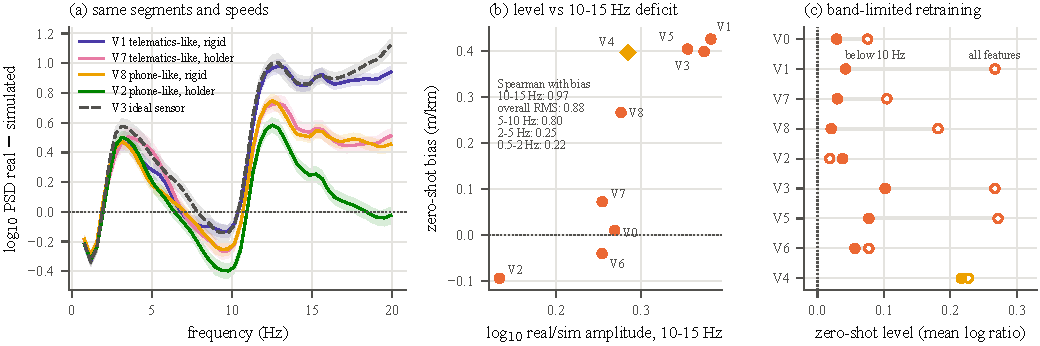
\includegraphics[width=\textwidth]{v3_spectra.pdf}
\caption{Simulated versus real vibration. (a) Welch power spectral density, real minus simulated (log$_{10}$), on the same segments in the same 10\,km/h speed bands for four sensor variants and the ideal sensor (bands: 95\,\% intervals, 1\,km-block bootstrap). (b) Zero-shot bias of the nine measured-profile variants against their real/simulated 10--15\,Hz amplitude ratio (diamond: V4, one vehicle), with the Spearman correlation of every band. (c) Mean zero-shot log level with all 13 features (open) and with the five features without vibration above 10\,Hz (filled).}
\label{fig:spectra}
\end{figure*}

\subsection{Where the simulated vibration differs}
\label{sec:res_mech}
On the same segments and speed bands, the real car vibrates more than every simulated variant at 2--5\,Hz (\spVoneMidPow--\spVfiveMidPow{} times the power) and like them at 5--10\,Hz, but above 10\,Hz the variants differ (Fig.~\ref{fig:spectra}a): at 10--15\,Hz the real car has \spVthreeHighPow{} and \spVoneHighPow{} times the power of the ideal and the rigid telematics-like sensor, yet only \spVtwoHighPow{} times that of the phone-like sensor with holder resonance.
Across the nine variants the zero-shot bias follows the amplitude deficit at 10--15\,Hz most closely (Spearman \baSpHighBias; Fig.~\ref{fig:spectra}b), but also that at 5--10\,Hz (\baSpMidHighBias) and of the overall RMS (\baSpRmsBias), and hardly those at 0.5--2 and 2--5\,Hz (\baSpLowBias, \baSpMidBias).
V4 departs from this pattern: its 10--15\,Hz ratio is close to V0's (\vpVfourRatioHigh{} vs \vpVzeroRatioHigh), its bias is not (\vvVfourBias{} vs \vrSimVzeroBias\,m/km).

To test which inputs carry these differences, we retrained every variant on the five features without vibration above 10\,Hz.
Over the eight sensor variants, the spread of the mean log level fell from \blFullSpreadLvl{} to \blLowSpreadLvl{} (\blRatioLvl\,\%; Fig.~\ref{fig:spectra}c), whereas dropping only the 10--15\,Hz band changed it by at most \blNoHighMaxChange\,\%: the sensor variants differ through all features that carry vibration above 10\,Hz.
The low-band estimator is less accurate (pooled MAE after a 5\,km level offset \blLowCalMin--\blLowCalMax{} instead of \blFullCalMin--\blFullCalMax\,m/km), and V4 stays outside the range of the sensor variants, so the vehicle population sets part of the level independently.
This test acts on the estimator's inputs; the physical source of the car's extra vibration above 10\,Hz, where its empirical transmissibility peaks (\invPeakHz\,Hz), is not identified, and the linear half-car omits candidates such as local modes of the console mount, tyre and suspension nonlinearity, drivetrain vibration and roll.
The simulated vibration also grows faster with speed than the real car's on the same roads (elasticity \ssSimUrbanMin--\ssSimUrbanMax{} vs \ssRealUrban{} on urban and \ssSimMotorwayMin--\ssSimMotorwayMax{} vs \ssRealMotorway{} on motorway segments), for every variant.

\begin{figure*}[t]
\centering
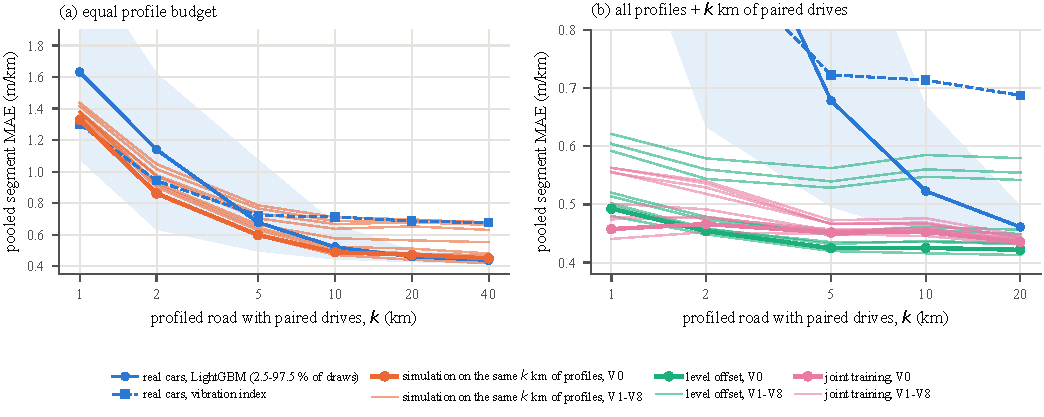
\includegraphics[width=\textwidth]{v3_value.pdf}
\caption{Simulation against paired real drives on the same 20 draws of $k$\,km of training-route road (pooled segment MAE on the held-out routes, means over draws; bold: V0, thin: V1--V8). Blue: real-only LightGBM (band: 2.5--97.5\,\% of draws) and vibration index (dashed). (a) LightGBM on simulated passes over the profiles of the same $k$\,km. (b) Simulation over all training-route profiles combined with the paired passes by a level offset (green) or joint training (pink); real-only values at 1 and 2\,km lie above the axis (LightGBM \vbRealOnlyOne{} and \vbRealOnlyTwo, index \vbRealIdxOne{} and \vbRealIdxTwo\,m/km).}
\label{fig:value}
\end{figure*}

\subsection{How much paired real data is needed}
\label{sec:res_value}
Fig.~\ref{fig:value} compares simulation with real drives on the same draws of $k$\,km (every variant and the test-route intervals: Supplement~\ref{S-sec:s_variants}).
Simulated drives over the profiles of the $k$\,km alone are no general substitute for the real drives over them (Fig.~\ref{fig:value}a): from 5\,km on, their value depends on the variant (\pcSameDiffTwentyMin{} to \pcSameDiffTwentyMax\,m/km against real-only LightGBM at 20\,km).
Simulated drives over all profiled training roads, combined with the paired passes, are a substitute (Fig.~\ref{fig:value}b).
With 5\,km of paired drives, every variant beats LightGBM trained on those drives alone (pooled MAE \vbRealOnlyFive\,m/km), with a level offset (\pcCalMaeFiveMin--\pcCalMaeFiveMax\,m/km, better in \pcCalWinsFiveMin--\pcCalWinsFiveMax{} of 20 draws) or with joint training (\poMaeFiveMin--\poMaeFiveMax\,m/km, better in \poWinsFiveRange{} of 20 draws), and the block-bootstrap intervals over the test routes exclude zero for every variant and both methods.
The reference simulator with a 5\,km offset (\vvVzeroCalFive\,m/km, \vvVzeroCalFiveLo--\vvVzeroCalFiveHi{} over draws) is more accurate than 20\,km (\vbRealOnlyTwenty) or 40\,km (\vbRealOnlyForty\,m/km) of real drives alone.
One pass per segment suffices: with \pdUnitsOne{} instead of \kdUnitsFive{} segment-passes, the simulation-based estimates hardly change (\pdCalOneMin--\pdCalOneMax{} and \pdPoolOneMin--\pdPoolOneMax\,m/km) and stay better than real-only training \pdOneAllDraws, whose error rises to \pdRealOne\,m/km.
An index with the car's own speed exponent and an affine fit to the same 5\,km reaches only \nsCarAffineFive\,m/km, so simulation contributes more than a speed normalisation.

With more paired data the two methods diverge.
Real-only training overtakes the level offset for V1, V3 and V5, the variants with the largest 10--15\,Hz deficit (the offset wins \pcCalHiDefWinsTwentyMax{} of 20 draws at 20\,km; differences \cuCalVoneTwenty{} to \cuCalVfiveTwenty\,m/km), while joint training stays better for every variant (\poDiffTwentyMin{} to \poDiffTwentyMax\,m/km at 20\,km, \poWinsTwentyRange{} of 20 draws, all intervals below zero), though not on every route (worse in \poRouteTwentyPos{} of \poRouteTwentyCells{} variant--route combinations, by at most \poRouteTwentyDiffMax\,m/km).
The reason is the kind of level error: an offset removes a common level and leaves the difference between the motorway and urban levels, which ranges from \ldSpreadMin{} to \ldSpreadMax{} over the variants and orders their MAE after the offset (Spearman \ldSpreadCalRho).
At 5\,km, joint training minus offset is \poLoDefDiffCalFiveMin{} to \poLoDefDiffCalFiveMax\,m/km for the six variants with small class differences and \poHiDefDiffCalFiveMin{} to \poHiDefDiffCalFiveMax\,m/km for V1, V3 and V5; with joint training the nine variants span only \poMaeSpreadFive\,m/km at 5\,km and \poMaeSpreadTwenty\,m/km at 20\,km, against \poCalSpreadFive{} and \poCalSpreadTwenty\,m/km with an offset.
